\documentclass[preprint,12pt,review,authoryear]{elsarticle}

\usepackage{graphicx}
\usepackage{titling}
\usepackage{setspace}
\usepackage{fancyhdr}
\usepackage[headheight=15pt]{geometry}
\usepackage{tikz}
\usepackage{xcolor}
\usepackage{mathptmx}
\usepackage{ragged2e}
\usepackage[pages=all]{background}
\usepackage{docmute}
\usepackage{graphicx}
\usepackage{pdflscape}
\usepackage{longtable}
\usepackage{array}
\usepackage{pdfpages}
\usepackage{lettrine}
\usepackage{tabularx, booktabs}

\usetikzlibrary{calc, arrows.meta,shapes.geometric,positioning,shadows.blur,trees}

\title{STU-Jamie_Pinnington_Individual_Project_40 Document}
\author{Jamie Pinnington}
\date{October 28, 2023}

\geometry{
    a4paper,
    total={170mm,257mm},
    left=20mm,
    top=20mm,
}

\definecolor{Border}{RGB}{72, 36, 107} % Border line colour

\backgroundsetup{% Add this block
scale=1,
color=black,
opacity=1,
angle=0,
contents={%

\begin{tikzpicture}[remember picture,overlay]
\draw[line width=2pt, Border] ($(current page.north west)+(1cm,-1cm)$) rectangle ($(current page.south east)+(-1cm,1cm)$);
\end{tikzpicture}% Add 'background lines'
}
}

\fancypagestyle{customStyle}{%
    \fancyhf{}  % Clear all header and footer fields
    \fancyhead[R]{\thepage}  % Place the page number in the top right
    \renewcommand{\headrulewidth}{0pt}  % Remove the header rule
    \setlength{\headheight}{14.49998pt}
}

\begin{document}

\pagestyle{customStyle} % Apply the custom style to all pages

% titlePage
\begin{titlepage} % title page
    
\begin{tikzpicture}[remember picture,overlay]
        \draw[line width=2pt, Border] ($(current page.north west)+(1cm,-1cm)$) rectangle ($(current page.south east)+(-1cm,1cm)$);
    \end{tikzpicture}
    \begin{flushright}
        \vspace*{0.1cm}
        \begin{tabular}{@{}p{6cm}@{}}
            {\fontfamily{ptm}\selectfont \small\textbf{FAO \textit{Dr. Amina Souag, Dr. Hannan Azhar}} \par}
        \end{tabular}
    \end{flushright}
    \begin{center}
        {\fontfamily{ptm}\selectfont \textbf{???????} \par}
        \vspace{0.25cm}
        {\fontfamily{ptm}\selectfont \textbf{BSc (Hons.) Computer Science}\par}
        \vspace{0.25cm}
        {\fontfamily{ptm}\selectfont \textbf{2023-2024}\par}
        \vspace{0.25cm}
        {\fontfamily{ptm}\selectfont \textbf{Individual Project 40}\par}
        \vspace{0.5cm}
        {\fontfamily{ptm}\selectfont \textbf{Title:} \textit{?????}\par}
        \vspace{0.25cm}
        {\fontfamily{ptm}\selectfont \textbf{Author:} \textit{Jamie Pinnington}\par}
        \vspace{0.25cm}
        {\fontfamily{ptm}\selectfont \textbf{Supervisors:} \textit{Dr. Amina Souag, Dr. Hannan Azhar}\par}
        \vspace{0.25cm}
        {\fontfamily{ptm}\selectfont \textbf{Email:} \textit{JP878@canterbury.ac.uk}\par}
        \begin{tabular}{@{}p{12cm}@{}}
            {\fontfamily{ptm}\selectfont This report is submitted in partial fulfilment of the requirement for
            the BSc in \textit{Computer Science} at Canterbury Christ Church University\par}
        \end{tabular}
    \end{center}
    \begin{center}\begin{singlespace}\begin{tabular}{@{}p{15cm}@{}}
                {\fontfamily{ptm}\selectfont I declare that this report is my own original work containing no personal data as defined in
                the Data Protection Act (1998) and that I have read, understood and accept the University's
                regulations on plagiarism/intellectual property rights/research ethics (in particular the
                Research Governance Handbook) and the IP 40 Module Handbook.\par}
            \end{tabular}\end{singlespace}\end{center}
    \begin{center}\begin{singlespace}\begin{tabular}{@{}p{15cm}@{}}
                {\fontfamily{ptm}\selectfont \textcolor{red}{Further, I accept that digital and/or hard copies of my Individual Project 40, or parts thereof, may be made
                    available to other students, individuals and organisations after it has been marked.}\par}
            \end{tabular}\end{singlespace}\end{center}
    \begin{center}\begin{singlespace}\begin{tabular}{@{}p{15cm}@{}}
                {\fontfamily{ptm}\selectfont \textcolor{red}{Finally, I accept that no copy of my Individual Project 40 will ever be returned regardless of the circumstances.}\par}
            \end{tabular}\end{singlespace}\end{center}
    \begin{center}
        {\fontfamily{ptm}\selectfont Signed \textit{Jamie Pinnington}\par}
        \vspace{0.25cm}
        {\fontfamily{ptm}\selectfont Date of Submission: \textit{??????}\par}
    \end{center}
    % Bottom of the page
\end{titlepage}

\clearpage % page 1

\begin{abstract}
\end{abstract}

\section{Acknowledgements}

\clearpage % page 2

\tableofcontents
\clearpage % page 3

\listoffigures
\clearpage % page 4

\listoftables
\clearpage % page 5

\section{Introduction:}

\lettrine[lines=2]{T}{his}

\section{Literature Review:}
\section{Introduction}
\subsection{Background}
\begin{itemize}
    \item why is this topic (ASL) important? (e.g., accessibility, communication)

    \item what is the specific problem being addressed? (e.g., fingerspelling recognition) (bridges the gap in communication and enhances the learning/usage of ASL.) (makes ai more accessible to this audience?)
          ASL ,
    \item what is the impact of an AI recognizer for this problem? (e.g., enables real-time communication, improves accessibility, etc.) (can this effect broader technology?)
\end{itemize}

Sign language is the primary form of communication for the deaf and hard of hearing community. It allows communication when the spoken language is not possible, and or when the speaker or receiver is deaf or hard of hearing.
Depending on the situation, and like any language, it requires both parties to be fluent in the language to communicate effectively. However, this is not always the case. American Sign Language(ASL) is a complete, complex language that employs signs made with the hands and other movements, including facial expressions and postures of the body, and is used natively in the
United States of America and globally by many individuals. Whilst no attempt has officially been made to survey the language, and most current estimates are based off of historical surveys that prove to be inaccurate\cite{mitchellHowManyPeople2006}. It is estimated that there are over 1 million signers\cite{AmericanSignLanguage}, but others estimates are as high as 2 million\cite{mitchellHowManyPeople2006}.
ASL communicates through a variety of means including gestures, non-manual markers and lexical signs. The most understood are lexical vocabulary, each corresponding to a word or morpheme. Gestures and non-manual markers such as facial expression can complement and convey more interactive or meaningful lexical signs. Additional constructs include usage of space, role shifting and classifiers.

\subsection{Purpose}

\begin{itemize}
    \item what is the purpose of the review?
    \item (e.g., to identify the state of the art in ASL fingerspelling recognition)
    \item (to identify the challenges and opportunities in ASL fingerspelling recognition)
    \item (to identify the most promising techniques for ASL fingerspelling recognition)
    \item * primary purpose is to build our own model, but we need to know what's out there first. *

\end{itemize}
\subsection{Scope}
\begin{itemize}
    \item what is the scope of the review? (e.g., ASL fingerspelling recognition) (what is the scope of the problem? (e.g., real-time recognition of fingerspelling gestures) (what is the scope of the solution? (e.g., image-based recognition of fingerspelling gestures) (what is the scope of the evaluation? (e.g., accuracy, speed, etc.)
    \item what is the scope of the literature? (e.g., papers published in the last 5 years) (what is the scope of the sources? (e.g., peer-reviewed journal articles, conference papers, etc.)
    \item what we're not covering.
    \item only recognition and translation of ASL *fingerspelling* (not full ASL).
    \item specific the application/methodology (e.g., video-based recognition of fingerspelling gestures) (live/stream???)
\end{itemize}

\subsection{Research Questions}
\begin{itemize}
    \item RQ-1: Comparative Analysis of Machine Learning Models:
          What are the strengths and weaknesses of different machine learning models, such as Convolutional Neural Networks (CNNs), Recurrent Neural Networks (RNNs), and Transformer models, in the context of ASL fingerspelling recognition?
    \item RQ-2: Performance Evaluation:
          How do various machine learning models perform in terms of accuracy, processing speed, and reliability for ASL fingerspelling recognition under different conditions (e.g., varying lighting, hand positions, backgrounds)?
    \item RQ-3: Dataset and Model Suitability:
          How does the choice of dataset, including its size, diversity, and quality, influence the effectiveness of different machine learning models in recognizing ASL fingerspelling?
    \item RQ-4: Real-World Applications:
          Considering practical applications like kiosk systems, which machine learning models offer the best balance between technical performance and user experience for ASL fingerspelling recognition?
    \item RQ-5: Technical Challenges:
          What technical challenges are commonly faced across different machine learning models in ASL fingerspelling recognition, and how adaptable are these models to address such challenges?
    \item RQ-6: Impact of Environment Variables:
          To what extent do environmental variables (like hand orientation, motion speed, and background noise) affect the performance of different machine learning models in ASL fingerspelling recognition?
    \item RQ-7: State of the Art and future directions:
          What are the most recent and influential works in the field of ASL fingerspelling recognition, and what are the emerging trends and future directions?
\end{itemize}

\section{Methodology}

\subsection{Literature Identification}
This literature search was completed using the databases IEEE Xplore, Google Scholar, ACM Digital Library, and ScienceDirect. Search terms such as "ASL fingerspelling recognition", "Deep learning for ASL recognition",  "ASL recognition with CNN", "Accuracy of ASL recognition models", "Latest trends in ASL recognition", and "ASL recognition in real-time" were used alone and in conjunction with boolean operators "AND", "OR" to refine the search results. The search was limited to papers published in the last 5 years, and only peer-reviewed journal articles, conference papers, and high quality theses were considered. The search was also limited to papers written in English. The search was conducted in November 2023, and the results were filtered to include only papers that were published between 2018 and 2023.
\subsection{Literature Evaluation}
Of the literature that fit out search criteria, we selected the most relevant papers based on the following criteria: the relevance to the research questions, papers that specifically address ASL fingerspelling, machine learning models in sign language interpretation, papers that used widely recognized datasets relevant to ASL recognition, we chose to exclude editorials, opinion pieces, and non-peer reviewed articles. Papers also required a clear methodology, defined objectives and robust data analysis. Papers with high citation counts were also given preference.
\paragraph{Organizing and Categorizing}
This subsection describes how the selected literature was organized and categorized, providing the basis for a comprehensive synthesis.

\paragraph{Comparative Analysis}
A detailed comparative analysis of the methodologies and findings of the selected studies is presented here, highlighting similarities and differences in approaches.

\paragraph{Gaps and Trends}
This part identifies any gaps in the current research landscape and notes emerging trends in ASL fingerspelling recognition technology.

\paragraph{Conclusions and Narrative}
The conclusions drawn from the comparative analysis and their relation to the original research questions are discussed here, forming a narrative that captures the current state of the field.

\paragraph{Visual Representation and Critical Evaluation}

\begin{landscape}
    % !TeX root = main.tex
\newcolumntype{L}{>{\raggedright\arraybackslash}p{0.195\textwidth}}

\begin{footnotesize}
    \begin{longtable}{LLLLLLL} % Adjust the column width as needed
        \caption{Summary and Analysis of ASL Fingerspelling Recognition Models (2018-2023)}
        \label{table:asl-comparison}                                                                                                                                                                                                                                                                                                                                                                                                                                                                                                                                                                                                          \\
        \toprule
        Reference                                          & Model Used                                                                                                            & Framework                & Dataset                        & Key Findings                                                                                                                                              & Performance Metrics                                    & Challenges Addressed                                                                                                                                                    \\
        \midrule
        \endfirsthead
        \toprule
        Reference                                          & Model Used                                                                                                            & Framework                & Dataset                        & Key Findings                                                                                                                                              & Performance Metrics                                    & Challenges Addressed                                                                                                                                                    \\
        \midrule
        \endhead
        \bottomrule
        \endfoot
        \endlastfoot
        \cite{skumarTimeSeriesNeural2018}                  & RNN, LSTM, Attention, Encoder/Decoder                                                                                 & [Not Specified]          & NCSLGR Corpus                  & Recognition and translation of ASL glosses                                                                                                                & GRR: 86\%, GER: 23\%                                   & Real-time recognition and translation                                                                                                                                   \\

        \cite{weerasooriyaSinhalaFingerspellingSign2022}   & RF, KNN, LR                                                                                                           & [Not specified]          & FASSL custom dataset           & Developed a classifier for static signs using a small dataset                                                                                             & Accuracy: 87.9\% (correct estimates)                   & Pose classification with limited data                                                                                                                                   \\

        \cite{cihancamgozSignLanguageTransformers2020}     & Transformers with CTC loss                                                                                            & PyTorch                  & PHOENIX14T                     & State-of-the-art results in recognition and translation                                                                                                   & WER, BLEU-4 scores                                     & Translation from sign language videos to spoken language sentences                                                                                                      \\

        \cite{abiyevReconstructionConvolutionalNeural2020} & CNN, SSD, FCN                                                                                                         & [Not specified]          & Kaggle ASL Fingerspelling      & High accuracy, vision-based translation                                                                                                                   & Accuracy: 92.21\%                                      & Real-time translation, robustness in ASL recognition                                                                                                                    \\

        \cite{bantupalliAmericanSignLanguage2018}          & CNN, LSTM, RNN                                                                                                        & OpenCV                   & Self-created Dataset           & Effective recognition with custom CNN model                                                                                                               & Accuracy: 98.11\%                                      & Robust recognition in controlled environments                                                                                                                           \\

        \cite{kabadeAmericanSignLanguage2023}              & ResNet, Bi-LSTM, CTC, Attention                                                                                       & [Not specified]          & ChicagoFSWild                  & Recognition using optical flow and attention, preprocessing for occlusions                                                                                & Letter accuracy: 57\%                                  & Recognition in 'wild' conditions, occlusions                                                                                                                            \\

        \cite{shiAmericanSignLanguage2018}                 & CNN, LSTM, CTC                                                                                                        & Faster R-CNN             & Custom YouTube Dataset         & Improved accuracy with hand detection                                                                                                                     & Test Acc: 41.9\% with CTC                              & Recognition in the wild, varying conditions                                                                                                                             \\

        \cite{shiFingerspellingRecognitionWild2019}        & CNN, RNN, CTC, Attention                                                                                              & TensorFlow               & ChicagoFSWild, ChicagoFSWild+  & Enhanced recognition in uncontrolled environments                                                                                                         & Word Error Rate: 27.2                                  & Recognition in diverse and challenging real-world scenarios                                                                                                             \\

        \cite{shiFingerspellingDetectionAmerican2021}      & 2D/3D-CNN, Bi-LSTM                                                                                                    & OpenPose                 & ChicagoFSWild, ChicagoFSWild+  & Superior detection in uncontrolled environments                                                                                                           & AP@IoU: 0.495, MSA: 0.386                              & Handling fine-grained handshapes and signer’s pose                                                                                                                      \\

        \cite{nguyenDeepLearningAmerican2019}              & 1) LBP, HOG descriptors, multi-class SVM, 2) End-to-end CNN 3) CNN weights as feature extractor for Linear-kernel SVM & [Not specified]          & Massey Dataset                 & Three diverse methods for fingerspelling recognition                                                                                                      & Recognition rate: 97.49\%, 98.23\%, 98.30\%            & Adaptability in feature extraction and classification approaches                                                                                                        \\

        \cite{chongAmericanSignLanguage2018}               & SVM and DNN                                                                                                           & TensorFlow, Scikit-learn & Self-created Dataset           & Comparison of SVM and DNN for ASL recognition; effective use of LOO approach for bias avoidance                                                           & Recognition rate: 72.79\%, 88.79\%                     & Multi-class classification with 36 classes (26 letters and 10 digits)                                                                                                   \\

        \cite{bantupalliAmericanSignLanguage2018}          & CNN (Inception) for spatial features, LSTM for temporal features                                                      & TensorFlow, Keras        & American Sign Language Dataset & Efficient extraction of temporal and spatial features; use of Inception and LSTM models                                                                   & Accuracy up to 93\% (Softmax Layer), 58\% (Pool Layer) & Managing longer sequences with LSTM; preventing overfitting with dropout                                                                                                \\

        \cite{shiSearchingFingerspelledContent2022}        & FSS-Net (End-to-End Model for Fingerspelling Detection and Text Matching)                                             & [Not Specified]          & ChicagoFSWild, ChicagoFSWild+  & Introduced explicit temporal localization for fingerspelling search and retrieval. Demonstrated effective fingerspelling detection in varying conditions. & mAP: 0.684 (YouTube), 0.584 (DeafVIDEO), 0.629 (Misc)  & Fingerspelling detection in diverse visual conditions; handling open vocabulary and arbitrary-length queries; confusion between similar handshapes; detection failures. \\

        \cite{gajurelFineGrainedVisualAttention2021}       & Fine-Grained Visual Attention with Transformer Model (CTC, CNN, LSTM)                                                 & [Not specified]          & ChicagoFSWild                  & Significantly improved state-of-the-art performance in fingerspelling recognition using Transformer-based contextual attention mechanism                  & Letter Accuracy: 46.96 \% (dev), 48.36\% (test)        & Addressed challenges in capturing fine-grained details in unsegmented continuous video data. Focused on improving generalization and regularization of the model.       \\

        \bottomrule
    \end{longtable}
\end{footnotesize}
\end{landscape}

\subsection{Report Structure}
- what is the structure of the report? (e.g., introduction, literature review, etc.) (aka roadmap?)

\subsection{Conclude Introduction}

\begin{itemize}
    \item By understanding, the insight gained from this review will be used to inform the design and implementation of our own model.
    \item * evidence based approach is neccessary to be impactful *

\end{itemize}
\section{Historical Context} % RQ-7
\begin{itemize}
    \item Evolution of ASL fingerspelling recognition
    \item Major milestones and breakthroughs
\end{itemize}

\section{Methods and Techniques} % RQ-1, RQ-2, RQ-3
\begin{itemize}
    \item Overview of methods used in the literature
    \item Image/Video-based Approaches
    \item Framework-based Approaches (e.g., MediaPipe)
    \item Hybrid methods
    \item Evaluation metrics commonly used
\end{itemize}

\section{Challenges in ASL Fingerspelling Recognition} % RQ-5, RQ-6
\begin{itemize}
    \item Technical challenges (e.g., diverse handshapes, background noise)
    \item Data challenges (e.g., lack of large labeled datasets)
    \item Real-world challenges (e.g., different lighting conditions, user variability)
\end{itemize}

\section{Overcoming Obstacles} % RQ-5
\begin{itemize}
    \item Techniques to enhance accuracy
    \item Data augmentation strategies
    \item Transfer learning and pre-trained models
\end{itemize}

\section{State of the Art/Real-World Applications} % RQ-4, RQ-7
\begin{itemize}
    \item Most recent and influential works in the field
    \item Comparison of different methods' performance
    \item Real-world applications and success stories
\end{itemize}

\section{Future Directions and Open Challenges} % RQ-7
\begin{itemize}
    \item Emerging trends in the field
    \item Areas that need further research
    \item Potential impact of advancements (e.g., in deep learning)
\end{itemize}

\section{Ethical and Societal Considerations}
\begin{itemize}
    \item Data privacy concerns
    \item Bias and fairness in ASL recognition models
    \item Implications for the deaf and hard of hearing community

\end{itemize}

\section{Main Conclusion}
\begin{itemize}
    \item Summary of the main findings of the review
    \item Reiteration of the importance of the topic
\end{itemize}

\bibliographystyle{elsarticle-harv}
\bibliography{library}

% MAIN CHAPTERS
\section{MAIN CHAPTERS:}
\subsection{Chapter 1:}

\section{DEVELOPMENT NOTES}

\subsection{Algorithm Pseudocode}
https://ctan.math.washington.edu/tex-archive/macros/latex/contrib/algpseudocodex/algpseudocodex.pdf

\subsection{Model Art}
https://github.com/ashishpatel26/Tools-to-Design-or-Visualize-Architecture-of-Neural-Network?tab=readme-ov-file

\appendix{Appendices}
\newpage
\onecolumn
\section{Glossary}
\pagenumbering{arabic} % Reset page numbering
\renewcommand{\thepage}{A\arabic{page}}
\newpage
\section{Marking Scheme}
\pagenumbering{arabic} % Reset page numbering
\renewcommand{\thepage}{B\arabic{page}}
\newpage
\section{Changes to the Project Initiation Document}
\pagenumbering{arabic} % Reset page numbering
\renewcommand{\thepage}{C\arabic{page}}
\newpage
\section{Current Environment Investigation Report}
\pagenumbering{arabic} % Reset page numbering
\renewcommand{\thepage}{D\arabic{page}}
\newpage
\section{Requirements Specification}
\pagenumbering{arabic} % Reset page numbering
\renewcommand{\thepage}{E\arabic{page}}
\newpage
\section{Design Report}
\pagenumbering{arabic} % Reset page numbering
\renewcommand{\thepage}{F\arabic{page}}
\newpage
\section{Implementation}
\pagenumbering{arabic} % Reset page numbering
\renewcommand{\thepage}{G\arabic{page}}
\newpage
\section{Testing}
\pagenumbering{arabic} % Reset page numbering
\renewcommand{\thepage}{H\arabic{page}}
\newpage
\section{User Guide}
\pagenumbering{arabic} % Reset page numbering
\renewcommand{\thepage}{I\arabic{page}}
\newpage
\section{Project Management}
\pagenumbering{arabic} % Reset page numbering
\renewcommand{\thepage}{J\arabic{page}} % Format page numbering as A1, A2, etc.
% Include the Work Breakdown Structure
\begin{figure}[ht]
    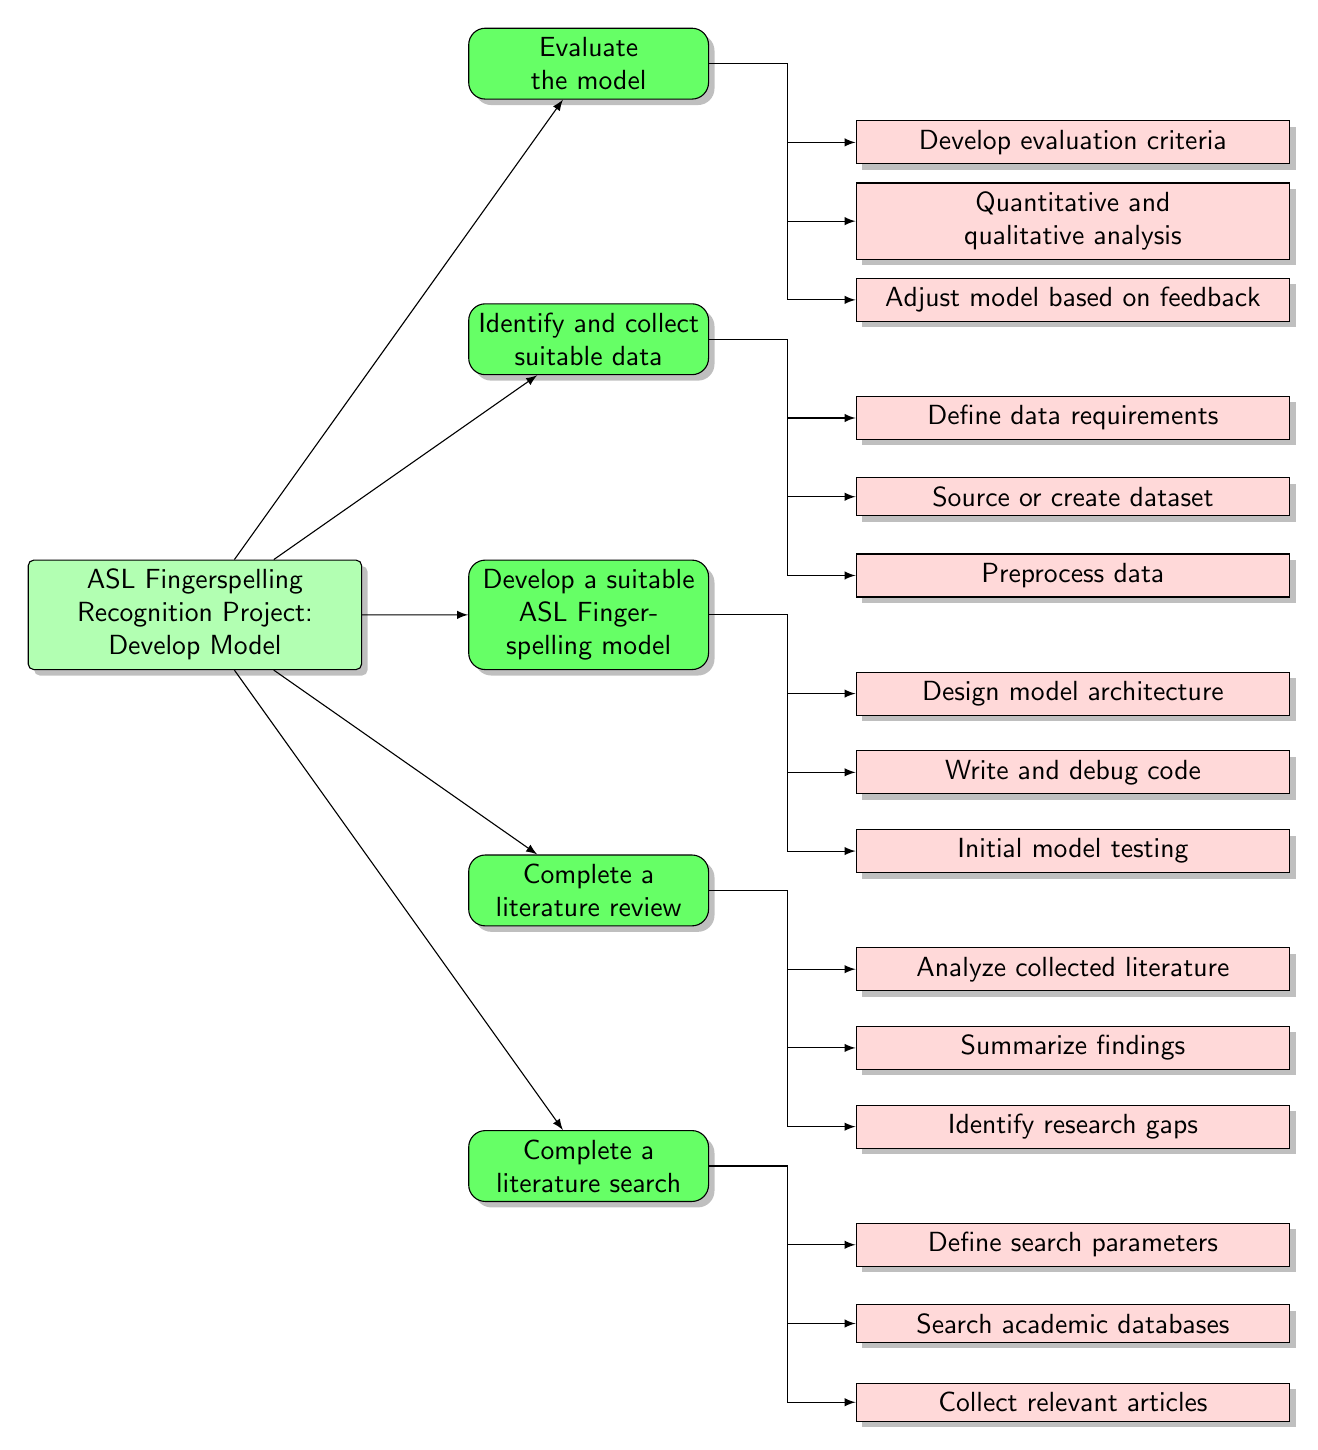
\begin{tikzpicture}[
                grow=right,
                level 1/.style={sibling distance=35mm, level distance=50mm},
                level 2/.style={sibling distance=35mm, level distance=40mm},
                level 3/.style={sibling distance=35mm, level distance=40mm},
                edge from parent/.style={->,draw},
                >=latex]
        \tikzset{
                basic/.style  = {draw, text width=4cm, drop shadow, font=\sffamily, rectangle},
                root/.style   = {basic, rounded corners=2pt, thin, align=center,
                                fill=green!30},
                level 2/.style = {basic, rounded corners=6pt, thin,align=center, fill=green!60,
                                text width=8em},
                level 3/.style = {basic, thin, align=center, fill=pink!60, text width=15em}
        }
        % root of the the initial tree, level 1
        \node[root] {ASL Fingerspelling Recognition Project: Develop Model}
        % The first level, as children of the initial tree
        child {node[level 2] (c1) {Complete a literature search}}
        child {node[level 2] (c2) {Complete a literature review}}
        child {node[level 2] (c3) {Develop a suitable ASL Fingerspelling model}}
        child {node[level 2] (c4) {Identify and collect suitable data}}
        child {node[level 2] (c5) {Evaluate the model}};

        % The second level, relatively positioned nodes
        \begin{scope}[every node/.style={level 3}]
                % Tasks for Complete a literature search
                \node [below of = c1, xshift=175pt] (c11) {Define search parameters};
                \node [below of = c11] (c12) {Search academic databases};
                \node [below of = c12] (c13) {Collect relevant articles};

                % Tasks for Complete a literature review
                \node [below of = c2, xshift=175pt] (c21) {Analyze collected literature};
                \node [below of = c21] (c22) {Summarize findings};
                \node [below of = c22] (c23) {Identify research gaps};

                % Tasks for Develop a suitable ASL Fingerspelling model
                \node [below of = c3, xshift=175pt] (c31) {Design model architecture};
                \node [below of = c31] (c32) {Write and debug code};
                \node [below of = c32] (c33) {Initial model testing};

                % Tasks for Identify and collect suitable data
                \node [below of = c4, xshift=175pt] (c41) {Define data requirements};
                \node [below of = c41] (c42) {Source or create dataset};
                \node [below of = c42] (c43) {Preprocess data};

                % Tasks for Evaluate the model
                \node [below of = c5, xshift=175pt] (c51) {Develop evaluation criteria};
                \node [below of = c51] (c52) {Quantitative and qualitative analysis};
                \node [below of = c52] (c53) {Adjust model based on feedback};
        \end{scope}

        % lines from each level 1 node to every one of its "children"
        % Continuous lines for each node without an arrow at the fork
        \foreach \parent in {1,...,5} {
                        % Draw a line to the fork point without an arrow
                        \path (c\parent.east) -- +(10mm,0) coordinate (fork\parent);
                        \draw (c\parent.east) -- (fork\parent);

                        % Create branches from the fork to each child with an arrow
                        \foreach \value in {1,2,3} {
                                        \draw[->] (fork\parent) |- (c\parent\value.west);
                                }
                };


\end{tikzpicture}



    \caption{Work Breakdown Structure: Develop Model}
    \label{fig:WBS: Develop Model}
\end{figure}
\newpage
\begin{landscape}
    \begin{figure}[ht]
        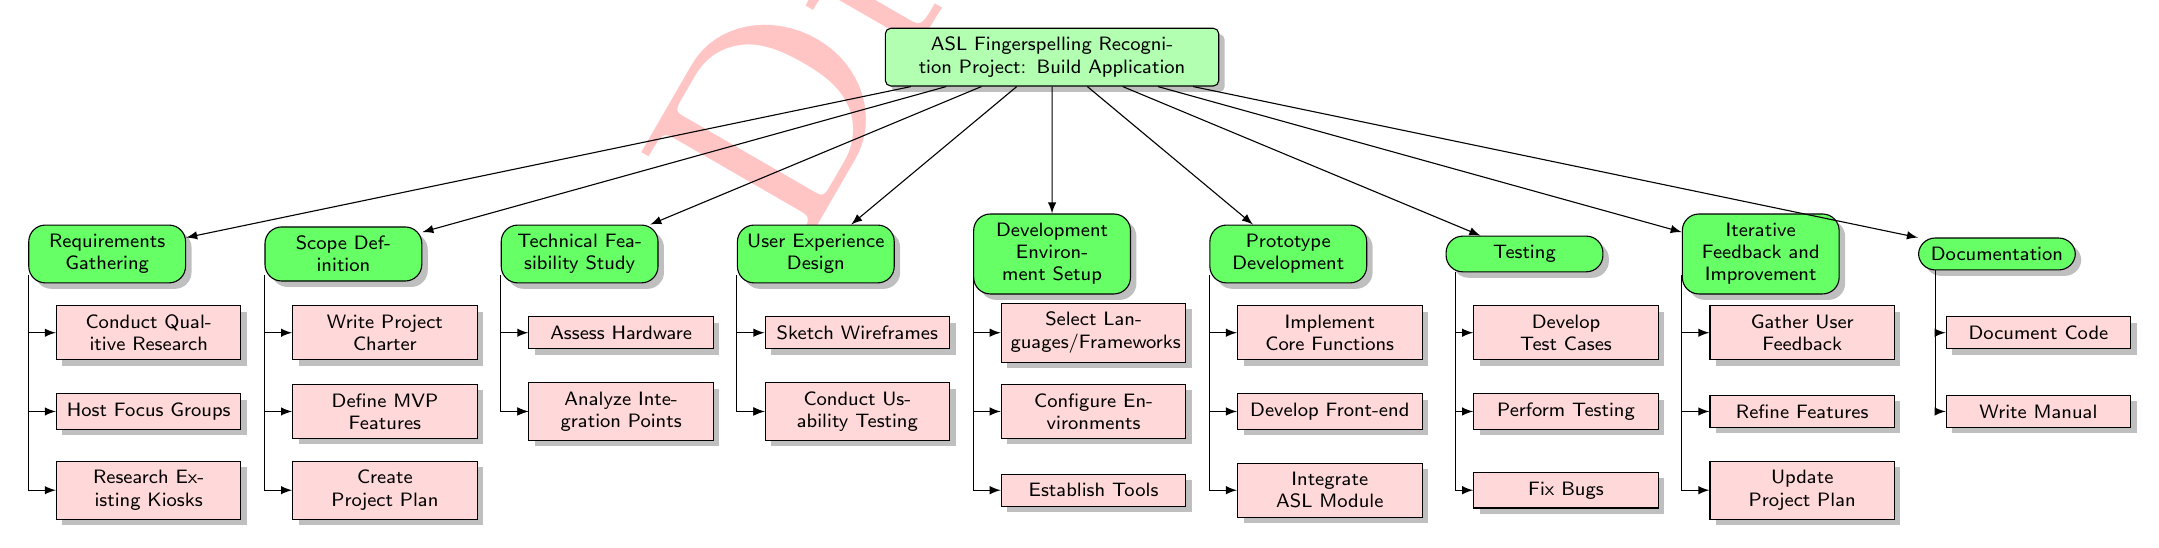
\begin{tikzpicture}[
                level 1/.style={sibling distance=30mm, level distance=25mm},
                level 2/.style={sibling distance=15mm},
                level 3/.style={sibling distance=15mm},
                edge from parent/.style={->,draw},
                >=latex]
        \tikzset{
                basic/.style  = {draw, text width=4cm, drop shadow, font=\sffamily\scriptsize, rectangle},
                root/.style   = {basic, rounded corners=2pt, thin, align=center,
                                fill=green!30},
                level 2/.style = {basic, rounded corners=6pt, thin,align=center, fill=green!60,
                                text width=5em},
                level 3/.style = {basic, thin, align=center, fill=pink!60, text width=6em}
        }
        % root of the the initial tree, level 1
        \node[root] {ASL Fingerspelling Recognition Project: Build Application}
        % The first level, as children of the initial tree
        child {node[level 2] (c1) {Requirements Gathering}}
        child {node[level 2] (c2) {Scope Definition}}
        child {node[level 2] (c3) {Technical Feasibility Study}}
        child {node[level 2] (c4) {User Experience Design}}
        child {node[level 2] (c5) {Development Environment Setup}}
        child {node[level 2] (c6) {Prototype Development}}
        child {node[level 2] (c7) {Testing}}
        child {node[level 2] (c8) {Iterative Feedback and Improvement}}
        child {node[level 2] (c9) {Documentation}};

        % The second level, relatively positioned nodes
        \begin{scope}[every node/.style={level 3}]
                % Tasks for Requirements Gathering
                \node [below of = c1, xshift=15pt] (c11) {Conduct Qualitive Research};
                \node [below of = c11] (c12) {Host Focus Groups};
                \node [below of = c12] (c13) {Research Existing Kiosks};

                % Tasks for Scope Definition
                \node [below of = c2, xshift=15pt] (c21) {Write Project Charter};
                \node [below of = c21] (c22) {Define MVP Features};
                \node [below of = c22] (c23) {Create Project Plan};

                % Tasks for Technical Feasibility Study
                \node [below of = c3, xshift=15pt] (c31) {Assess Hardware};
                \node [below of = c31] (c32) {Analyze Integration Points};

                % Tasks for User Experience Design
                \node [below of = c4, xshift=15pt] (c41) {Sketch Wireframes};
                \node [below of = c41] (c42) {Conduct Usability Testing};

                % Tasks for Development Environment Setup
                \node [below of = c5, xshift=15pt] (c51) {Select Languages/Frameworks};
                \node [below of = c51] (c52) {Configure Environments};
                \node [below of = c52] (c53) {Establish Tools};

                % Tasks for Prototype Development
                \node [below of = c6, xshift=15pt] (c61) {Implement Core Functions};
                \node [below of = c61] (c62) {Develop Front-end};
                \node [below of = c62] (c63) {Integrate ASL Module};

                % Tasks for Testing
                \node [below of = c7, xshift=15pt] (c71) {Develop Test Cases};
                \node [below of = c71] (c72) {Perform Testing};
                \node [below of = c72] (c73) {Fix Bugs};
                % Tasks for Iterative Feedback and Improvement
                \node [below of = c8, xshift=15pt] (c81) {Gather User Feedback};
                \node [below of = c81] (c82) {Refine Features};
                \node [below of = c82] (c83) {Update Project Plan};

                % Tasks for Documentation
                \node [below of = c9, xshift=15pt] (c91) {Document Code};
                \node [below of = c91] (c92) {Write Manual};
        \end{scope}

        % lines from each level 1 node to every one of its "children"
        % Loop over each parent
        % Loop over each parent
        \foreach \parent in {1,...,9} {
                        % Draw lines to child nodes that have been defined
                        \draw[->] (c\parent.195) |- (c\parent1.west);
                        \draw[->] (c\parent.195) |- (c\parent2.west);
                        % Check for exceptions with different number of children
                        \ifnum\parent=9
                                % Parent 9 only has 2 children
                        \else
                                \ifnum\parent=4
                                        % Parent 4 has 4 children
                                        \draw[->] (c\parent.195) |- (c\parent2.west);
                                \else
                                        \ifnum\parent=3
                                                % Parent 3 has 4 children
                                                \draw[->] (c\parent.195) |- (c\parent2.west);
                                        \else
                                                % All other parents have 3 children
                                                \draw[->] (c\parent.195) |- (c\parent3.west);
                                        \fi
                                \fi
                        \fi
                }
\end{tikzpicture}

        \caption{Work Breakdown Structure: Build Application}
        \label{fig:WBS: Build Application}
    \end{figure}
\end{landscape}
\newpage
\begin{figure}[ht]
    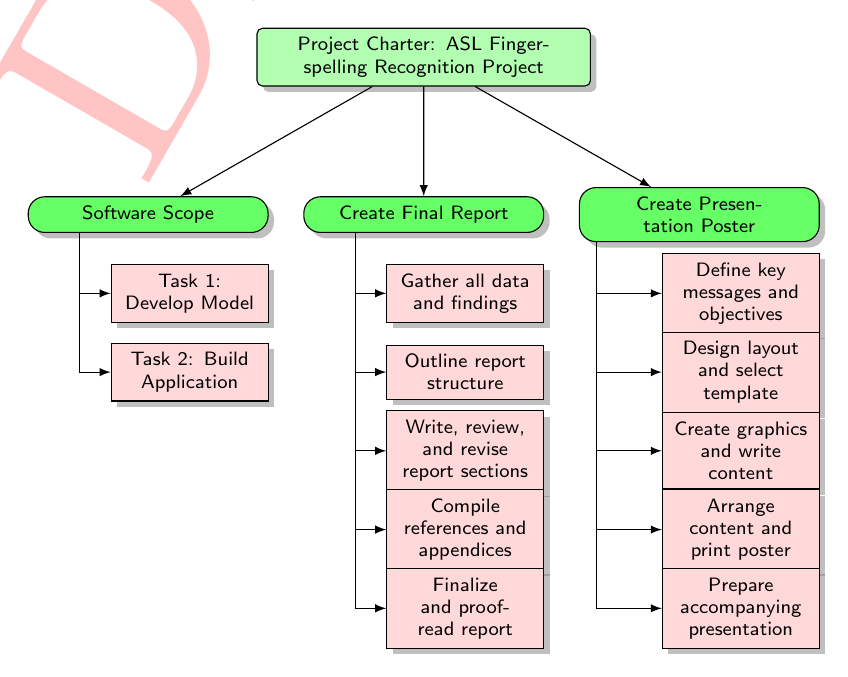
\begin{tikzpicture}[
                level 1/.style={sibling distance=35mm, level distance=20mm},
                level 2/.style={sibling distance=25mm, level distance=20mm},
                level 3/.style={sibling distance=35mm, level distance=20mm},
                edge from parent/.style={->,draw},
                >=latex]
        \tikzset{
                basic/.style  = {draw, text width=4cm, drop shadow, font=\sffamily\scriptsize, rectangle},
                root/.style   = {basic, rounded corners=2pt, thin, align=center,
                                fill=green!30},
                level 2/.style = {basic, rounded corners=6pt, thin,align=center, fill=green!60,
                                text width=8em},
                level 3/.style = {basic, thin, align=center, fill=pink!60, text width=5em}
        }
        % root of the the initial tree, level 1
        \node[root] {Project Charter: ASL Fingerspelling Recognition Project}
        % The first level, as children of the initial tree
        child {node[level 2] (c1) {Software Scope}}
        child {node[level 2] (c3) {Create Final Report}}
        child {node[level 2] (c4) {Create Presentation Poster}};

        % The second level, relatively positioned nodes
        \begin{scope}[every node/.style={level 3}]
                % Tasks for Complete a literature search
                \node [below of = c1, xshift=15pt] (c11) {Task 1: Develop Model};
                \node [below of = c11] (c12) {Task 2: Build Application};

                % Tasks for Create Final Report
                \node [below of = c3, xshift=15pt] (c31) {Gather all data and findings};
                \node [below of = c31] (c32) {Outline report structure};
                \node [below of = c32] (c33) {Write, review, and revise report sections};
                \node [below of = c33] (c34) {Compile references and appendices};
                \node [below of = c34] (c35) {Finalize and proofread report};

                % Tasks for Create Presentation Poster
                \node [below of = c4, xshift=15pt] (c41) {Define key messages and objectives};
                \node [below of = c41] (c42) {Design layout and select template};
                \node [below of = c42] (c43) {Create graphics and write content};
                \node [below of = c43] (c44) {Arrange content and print poster};
                \node [below of = c44] (c45) {Prepare accompanying presentation};
        \end{scope}

        % lines from each level 1 node to every one of its "children"
        % Continuous lines for each node without an arrow at the fork

        \foreach \value in {1,2}
        \draw[->] (c1.195) |- (c1\value.west);

        \foreach \value in {1,...,5}
        \draw[->] (c3.195) |- (c3\value.west);

        \foreach \value in {1,...,5}
        \draw[->] (c4.195) |- (c4\value.west);

\end{tikzpicture}



    \caption{Work Breakdown Structure}
    \label{fig:WBS: Project Charter}
\end{figure}
\newpage
\begin{landscape}
    \begin{figure}[ht]
        \centering
        % Placeholder for the Gantt chart
        \fbox{\parbox{15cm}{\centering Gantt chart placeholder \\ (Refer to the accompanying zipped file for the full chart)}}
        \caption{Gantt Chart}
        \label{fig:GanttChart}
    \end{figure}
    In this report's accompanying zipped file, a detailed Gantt chart is included as a separate document. Due to its extensive size and complexity, it is provided as an individual file to facilitate detailed review and ensure clarity. Please refer to the zipped file named gantt-project.png for the complete Gantt chart, which offers an in-depth view of the project timeline and milestones.
\end{landscape}
\begin{figure}[ht]
    \begin{longtable}{|>{\raggedright\arraybackslash}p{3cm}|>{\raggedright\arraybackslash}p{3cm}|>{\raggedright\arraybackslash}p{2cm}|>{\raggedright\arraybackslash}p{2cm}|>{\raggedright\arraybackslash}p{3cm}|}
    \hline
    \textbf{Risk} & \textbf{Impact} & \textbf{Probability} & \textbf{Status} & \textbf{Mitigation Strategy} \\
    \hline
    \endhead
    % Risks here...
    Inaccurate ASL Recognition & High & Medium & Open & Enhance data collection and improve algorithm accuracy. \\
    \hline
    Data Privacy Concerns & High & High & Open & Implement GDPR compliant data handling processes. \\
    \hline
    Loss of Data & High & Low & Open & Implement GoogleDrive and GitHub repository. \\
    \hline
    Loss of Project Supervisor & High & Low & Open & Maintain regular communication with supervisor. \\
    \hline
    Project Delays & Medium & High & Open & Develop a schedule with buffers and regularly update it. \\
    \hline
    User Adoption Challenges & Medium & High & Open & Engage with users early and incorporate feedback. \\
    \hline
    Technology Integration Issues & Medium & Medium & Open & Conduct compatibility testing. \\
    \hline
\end{longtable}
    \caption{Risk register}
    \label{fig:Risk Register}
\end{figure}
\newpage
\section{Meetings With Supervisor}
\pagenumbering{arabic} % Reset page numbering
\renewcommand{\thepage}{K\arabic{page}}
\newpage
\begin{longtable}{|p{2cm}|p{2cm}|p{3cm}|p{4cm}|p{4cm}|}
    \hline
    \textbf{Date}    & \textbf{Time} & \textbf{Location} & \textbf{Purpose}                        & \textbf{Description and Actions}                                                                                                                                                   \\
    \hline
    \endhead
    15 November 2023 & 13:00 – 14:00 & CCCU - Lg33       & Discuss project and literature research & Reviewed current status, discussed challenges, and agreed on next steps including further research on ASL recognition and user-centric approach to requirements. Contact charities \\
    \hline
    29 November 2023 & 13:00 - 14:00 & CCCU - Lg33       & ?                                       & ?                                                                                                                                                                                  \\
    \hline
\end{longtable}
\section{Agile Development: Timebox 1}
\pagenumbering{arabic} % Reset page numbering
\renewcommand{\thepage}{L\arabic{page}}
\newpage
\section{Agile Development: Timebox 2}
\pagenumbering{arabic} % Reset page numbering
\renewcommand{\thepage}{M\arabic{page}}
\newpage
\section{Agile Development: Timebox 3}
\pagenumbering{arabic} % Reset page numbering
\renewcommand{\thepage}{N\arabic{page}}
\newpage

\end{document}